\newpage
\section {Билет 26. Конфиденциальные вычисления. Гомоморфное шифрование и многосторонние вычисления.}

\textbf{Конфиденциальные вычисления} используются в тех случаях, когда необходимо обеспечить защиту некой информации ввиду из-за законодательных запреты, коммерческой тайны и т.д. При этом:
\begin{itemize}
\item некоторые вычисления можно провести только в <<недоверенной среде>> (
например непроверенное оборудование или ПО),
\item некоторые вычисления требуют слияния данных сразу нескольких клиентов, соотвественно требуется обеспечить конфиденциальность данных между разными клиентами. 
\end{itemize}

\textbf{Примеры, требующие использования конфиденциальных вычислений}:
\begin{itemize}
	\item Осуществление некоторых вычислений в <<облаке>>.
	\item Конфиденциальный поиск. Выполнение поисковых запросов в такой форме, чтобы БД (например Google) не знал, какая информация ищется.
	\item Машинное обучение на совместных данных.
	\item Вычисление значения функций от секретных функций. Например <<задача о двух миллионерах>>\url{https://clck.ru/pq7Zm}
\end{itemize}

Для каждой из задач может быть реализован специальный алгоритм, реализующий обеспечивающий \textbf{конфиденциальность вычислений}. В качестве примера возьмем задачу о  машинном обучении на совместных данных, ее конфиденциальный вариант называется \textbf{федеративное обучение}. Если вкратце, то используется одна модель для обучения данных, но все данные остаются у их владельца. Например подсказки при вводе на клавиатуре телефонов на Android: модель используется одна, однако все данные и их обработка хранятся и осуществляются на телефоне пользователя, а не где-то на серверах Google. На сервера отправляется только часть данных, по которым нельзя узнать что вводил конкретный человек на конкретном телефоне.(на лекциях это не особо обсуждалось, подробнее почитать можно вот здесь \url{https://www.machinelearningmastery.ru/federated-learning-a-new-ai-business-model-ec6b4141b1bf/})

Для произвольной задачи обычно используются следующие подходы:
\begin{itemize}
	\item Гомоморфное шифрование
	\item Многосторонние вычисления
	\item Функциональное шифрование 
\end{itemize}

Рассмотрим подробнее каждый из подходов.
\subsection {Функциональное шифрование}
Так, в схеме \textbf{функционального шифрования} для функции $F(\cdot, \cdot)$ шифрователь с мастер-ключом генерирует ключ $s_k$, позволяющий вычислять функцию $F(k, \cdot)$ от зашифрованных данных так, что расшифровщик, зная зашифрованный текст $c$ от данных $x$ и ключа $s_k$, был способен вычислить $F(k, x)$, не имея возможности узнать что-либо кроме результата вычисления функции по $x$. Лектор сказал что особо не понимает как это все работает и не знает реальных примеров использования, так что если интересно то поподробнее можно почитать здесь: \url{https://habr.com/ru/post/482790/}, \url{https://clck.ru/pqCRB}.


\subsection{Гомоморфное шифрование}
\textbf{Гомоморфным шифрованием} называется раздел криптографии, который посвящен разработке алгоритмов допускающих выполнение вычислений над \textbf{шифротекстами}. В качестве криптографических протоколов используются как симметричные (с одним ключом), так и асимметричные (с открытым и закрытым ключом). \url{https://otus.ru/nest/post/726/}

В \textbf{гомоморфном шифровании} подразумевается, что мы можем производить вычисления от \textbf{шифротекстами} и что для произвольной \textbf{вычислимой} функции $f$ верно (Enc = Encryption = шифрование):
$$Enc(f(x, y)) = f(Enc(x), Enc(y))$$

Под \textbf{вычислимыми} функциями подразумеваются функции, которые можно задать с помощью схемы из элементов на Рис. \ref{fig:logicscheme} (Что в целом эквивалентно определениям из всяких Матлогов/ТДФ/Дискры и т.д)
\begin{figure}[H]
	\centering
	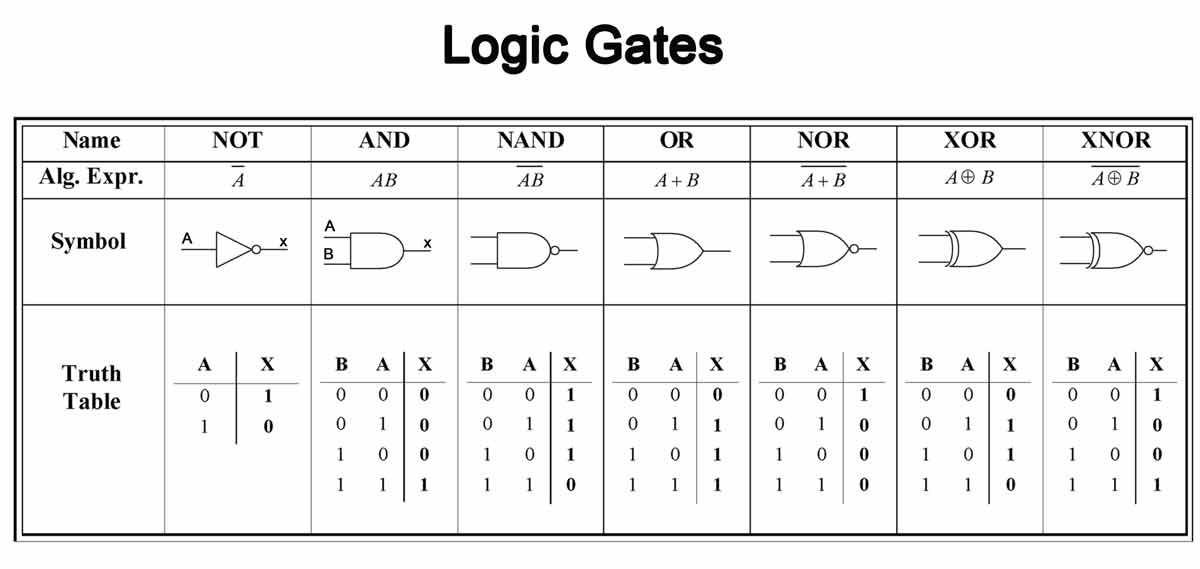
\includegraphics[scale = 0.3]{26/logic_cheme.jpeg}
	\caption{Логические элементы}
	\label{fig:logicscheme}
\end{figure}

Криптографическая схема состоит из 4х компонент:
\begin{enumerate}
	\item KeyGen - алгоритм создания открытого(PublicKey, $pk$) и закрытого (SecretKey, $sk$) ключей (RSA, DSA, Elgamal, и т.д.)
	\item Encryptioner - алгоритм шифрования, который по $pk$ создает \textbf{шифротекст} $c$ от исходных данных $x$: $c = Enc(pk, x)$
	\item Decryptioner - алгоритм дешифрования, который по $sk$ расшифровывает \textbf{шифротекст} $c$ от исходных данных $x$: $x = Dec(sk, c)$
	\item Evaluator - алгоритм, позволяющий вычислять булевы схемы.
\end{enumerate} 

Для булевой схемы $f$ с $k$ входами, произвольной пары $(pk, sk)$ и любого $(x_1, \dots, x_k) \in \{0;1\}^k$ должно выполняться следующее: $$Dec(sk, Eval(pk, f, c_1,c_2, \dots, c_k)) = f(x_1, \dots, x_k), \, c_i = Enc(pk, x_i)$$


Взломостойкость данного метода зависит от KeyGen, Enc и Dec. В настоящее время безопасность подобных методов с открытыми ключами строиться на вычислительной сложности разложении числа на простые множители. Пусть выбрано число $p \in \mathbb{Z}$ и случайные числа $q_1, \dots, q_n \in \mathbb{N}$. Вычислим значения $m_i=pq_i$. При достаточно большом $n$ можно эффективно восстановить $p$ по $m_i$: вычислив $gcd(m_1, \dots, m_n)$.  Однако данная задача легко решается с помощью квантовых компьютеров. Поэтому используется так называемый алгоритм \textbf{обучения с ошибками}. Считается, что если вместо точных значений $m_i$ известны значения $pq_i+r_i$, где $r_i \in \mathbb{Z}$, то такая задач является вычислительно сложной даже для квантового компьютера. На данном приеме строятся схемы \textbf{гомоморфного шифрования}.

Cхема простого \textbf{гомеоморфного шифрования}. В качестве секретного ключа $sk$ возьмем число $p \in \mathbb{N}$. Чем больше $p$ тем сложнее будет взломать данную схему.
\begin{itemize}
	\item Enc: для получения \textbf{шифротекста} $c_i$ с одного бита $b_i \in \{0, 1\}$ исходного сообщения вычислим $c_i = pq_i + 2r_i + b_i$, где $q_i$ и $r_i$ -- случайные числа, которые с равной вероятностью выбираются из определенных диапазонов.
	\item Dec: для расшифровывания \textbf{шифротекста} $c_i$ сначала вычисляется $c_i^{'} = (c_i \, mod \, p) \in (-p/2, p/2)$, а затем вычисляем $c_i \, mod \, 2$. Т.е $b_i = ((c_i \, mod \, p) \, mod \, 2)$. Под $a \, mod \, b $ подразумевается остаток от деления $a$ на $b$.
\end{itemize}


Если выполняется неравенство $|2r_i+b_i| < p/2$ (1), то $(c_i mod p) = 2r_i + b_i$, откуда следует корректность формулы для получения открытого текста.

Пусть заданы два \textbf{шифротекста} $c_1 = pq_1+2r_1+b_1, c_2 = pq_2+2r_2+b_2$, тогда их сумму $c = c_1+c_2 = pq_1+2r_1+b_1 + pq_2+2r_2+b_2$ можно представить в виде $p(q_1+q_2) + 2(r_1+r_2) + (b_1 + b_2)$, т.е $c$ является \textbf{шифротекстом} для $b_1 + b_2 \, mod \, 2$ с шумом $r_1 + r_2$. Аналогичным образом представляется произведение двух \textbf{шифротекстов}: $c = c_1 \cdot c_2 = (pq_1+2r_1+b_1)(pq_2+2r_2+b_2)$ с шумом $2r_1r_2 + b_1r_2 + b_2r_2$.

Как можно заметить при операции сложении шум растет медленнее чем при операции умножения, соотвественно при большом количестве операций и росте шума перестает выполняться (1) из-за чего дешифровка результата работы функции становиться невозможной. Решением данной проблемы является метод \textbf{самокорректировка (bootstrapping)}. Объяснение есть в этой статье \url{https://eprint.iacr.org/2021/091.pdf}.

\textbf{Примеры схем:}
\begin{itemize}
\item \textbf{BGV (Brakerski-Gentry-Vaikuntanathan)} - Схема ограниченного гомоморфного шифрования, позволяющая выполнять требуемое число арифметических операций над целыми числами без самокоррекции. 
\item \textbf{CKKS (Cheon, Kim, Kim, Song)} - Схема разработана для приближенных вычислений с комплексными числами.
\item \textbf{TFHE (Fast Fully Homomorphic Encryption over the Torus)} - Схема полного гомоморфного шифрования, которая реализует комбинацию логического элемента NAND (Рис. \ref{fig:logicscheme}) с последующей самокорректировкой. 
\end{itemize}

Быстродействие данных методов значительно хуже чем у методов с открытыми данными, примерно в $10^4-10^6$ раз медленнее. Сложение двух 32-битных значений методом \textbf{TFHE} занимает около 1 минуты, умножение 1.5 минуты, а целочисленное деление около 15 минут. Также стоит отметить, что не существует (и в теории не может существовать) <<гомоморфного>> языка программирования, так как невозможно реализовать даже такие базовые синтаксические конструкции как циклы и условные ветвления. 

\subsection{Многосторонние вычисления}
\textbf{Постановка задачи многосторонние вычислений}: участвуют $N$ участников $p_1, p_2, \dots, p_N$. У каждого участника есть тайные входные данные $x_1, x2, \dots, x_N$ соответственно. Участники хотят найти значение $f(d_1, d_2, \dots, d_N)$, где $f$ — известная всем участникам вычислимая функция от $N$ аргументов. Допускается, что среди участников будут получестные нарушители, то есть те, которые верно следуют протоколу, но пытаются получить дополнительную информацию из любых промежуточных данных. Требуется сохранить конфиденциальность входных параметров $x_i$. 

Далее подробно рассмотрим случаи для двух участников ($N=2$).
Тут можно использовать протокол \textbf{Oblivious Transfer (Забывчивая передача, Подробная реализация описана в вики \url{https://clck.ru/puQ3n})}, в котором отправитель передает по одной возможные части информации получателю, но не запоминает (является забывчивым), какие части были переданы, если вообще были. Отправитель имеет два значения $m_0, m_1$. Получатель выбирает $i \in \{0,1 \}$ и запрашивает у отправителя $m_i$ данные, при условии, что:
\begin{itemize}
	\item Получатель не получит данные $m_i-1$. То есть, если запрашиваем $m_0$, то точно не получим $m_1$ и наоборот.
	\item Отправитель не знает $i$, т.е. не знает что он отправил. 
\end{itemize}

\textbf{Oblivious Transfer} используется в одном из основных протоколов многосторонних вычислений -- \textbf{Garbled circuit
 (Искаженная схема) \url{https://ru.wikibrief.org/wiki/Garbled_circuit}, \url{https://en.wikipedia.org/wiki/Garbled_circuit}}. Опишем протокол:
\begin{enumerate}
	\item Базовая функция (например, у миллионеров) задача, функция сравнения) описывается как логическая схема с двумя входами. Схема известна обеим сторонам. Этот шаг может быть выполнен сторонним лицом.
	\item Алиса искажает (шифрует) схему. Мы называем Алису манипулятором.
	\item Алиса отправляет искаженную схему Бобу вместе со своим зашифрованным вводом.
	\item Для того, чтобы вычислить схему, Боб также должен искажать свой собственный ввод. Для этого ему нужна помощь Алисы. Потому что только мусорщик умеет зашифровать. Наконец, Боб может зашифровать свой ввод, не обращая внимания на передачу. В терминах определения, приведенного выше, Боб является получателем, а Алиса - отправителем при этой не обращающей внимания передаче. Именно в этом шаге используется \textbf{Oblivious Transfer}
	\item Боб оценивает (расшифровывает) схему и получает зашифрованные выходные данные. Мы называем Боба оценщиком.
	\item Алиса и Боб обмениваются данными для изучения вывода.
\end{enumerate}

